%%%%%%%%%%%%%%%%%%%%%%%%%%%%%%%%%%%%%%%%%%%%%%%%%%%%%%%%%%%%%%%%%%%
%                                                                 %
%   EPIO - Reference Manual -- LaTeX Source                       %
%                                                                 %
%   Main driver file. Includes other files of manual,             %
%   generates table of contents and includes index file.          %
%                                                                 %
%   Files referenced: epiofront.tex   front material              %
%                     epioch1.tex to epio10.tex                   %
%                     epiomain.ind   index made with makeindex    %
%                     cnasbibl.bib   bibliography files (BibTeX)  %
%                                                                 %
%   To run, you need the CERN styles cernman.sty and crnman11.sty %
%                                                                 %
%   Editor: Michel Goossens / CN-AS                               %
%   Last Mod.: 18 Nov 1993  23:15  mg                             %
%                                                                 %
%%%%%%%%%%%%%%%%%%%%%%%%%%%%%%%%%%%%%%%%%%%%%%%%%%%%%%%%%%%%%%%%%%%

\documentstyle[11pt,longtable,epsfig,makeidx]{cernman}
\setlongtables
\makeindex
\romanfont{times}
\def\condbreak#1{\par}
\PScommands% Initialize PS boxes
\setcounter{secnumdepth}{3}
\setcounter{tocdepth}{2}
\newmathalphabet*{\mathtt}{cmtt}{m}{n}
\newmathalphabet*{\mathbf}{cmr}{b}{n}
\begin{document}
%  ==================== Front material ============================
%%%%%%%%%%%%%%%%%%%%%%%%%%%%%%%%%%%%%%%%%%%%%%%%%%%%%%%%%%%%%%%%%%%
%                                                                 %
%   EPIO - Reference Manual -- LaTeX Source                       %
%                                                                 %
%   Front Material: Title page,                                   %
%                   Copyright Notice                              %
%                   Preliminary Remarks                           %
%                   Table of Contents                             %
%   EPS file      : cern15.eps, cnastit.eps                       %
%                                                                 %
%   Editor: Michel Goossens / CN-AS                               %
%   Last Mod.: 18 Nov 1993 22:45 mg                               %
%                                                                 %
%%%%%%%%%%%%%%%%%%%%%%%%%%%%%%%%%%%%%%%%%%%%%%%%%%%%%%%%%%%%%%%%%%%

%%%%%%%%%%%%%%%%%%%%%%%%%%%%%%%%%%%%%%%%%%%%%%%%%%%%%%%%%%%%%%%%%%%%
%    Tile page                                                     %
%%%%%%%%%%%%%%%%%%%%%%%%%%%%%%%%%%%%%%%%%%%%%%%%%%%%%%%%%%%%%%%%%%%%
\notHTML{\def\Ptitle#1{\special{ps: /Printstring (#1) def}
                       \epsfbox{/user/goossens/cnasall/cnastit.eps}}}
\HTML{\def\Ptitle#1{<B>#1</B>}}
 
\begin{titlepage}
\notHTML{\vspace*{-23mm}}%
\notHTML{\mbox{\epsfig{file=/usr/local/lib/tex/ps/cern15.eps,height=30mm}}}%
\HTML{<IMG SRC="../cernlogo.gif">}%
\hfill
\raise8mm\hbox{\Large\bf CERN Program Library Long Writeup I101}
\hfill\mbox{}
\HTML{<P>}
\begin{center}
\mbox{}\\[10mm]
\mbox{\Ptitle{EPIO}}\\[2cm]
\HTML{<P>\\}
{\LARGE Experimental Physics Input Output Package}\\[2cm]
\HTML{<P>\\}
{\LARGE User's Guide}\\[3cm]
\HTML{<P>\\}
{\Large Application Software and Databases Group}\\[1cm]
{\Large Computing and Networks Division}\\[2cm]
\end{center}
\HTML{<P>}
\notHTML{\vfill}%
\begin{center}\Large CERN Geneva, Switzerland\end{center}
\end{titlepage}

\Filename{H1Preface}
\HTML{<H1>Preface</H1>}

%%%%%%%%%%%%%%%%%%%%%%%%%%%%%%%%%%%%%%%%%%%%%%%%%%%%%%%%%%%%%%%%%%%%
%    Copyright  page                                               %
%%%%%%%%%%%%%%%%%%%%%%%%%%%%%%%%%%%%%%%%%%%%%%%%%%%%%%%%%%%%%%%%%%%%
\HTML{\PRE}
\thispagestyle{empty}
\framebox[\textwidth][t]{\hfill\begin{minipage}{0.96\textwidth}%
\vspace*{3mm}\begin{center}Copyright Notice\end{center}
\parskip\baselineskip
{\bf EPIO --- Experimental Physics Input Output Package}
 
CERN Program Library entry {\bf I101}
 
\copyright{} Copyright CERN, Geneva 1993
 
Copyright and any other appropriate legal protection of these
computer programs and associated documentation reserved in all
countries of the world.
 
These programs or documentation may not be reproduced by any
method without prior written consent of the Director-General
of CERN or his delegate.
 
Permission for the usage of any programs described herein is
granted apriori to those scientific institutes associated with
the CERN experimental program or with whom CERN has concluded
a scientific collaboration agreement.
 
Requests for information should be addressed to:
\vspace*{-.5\baselineskip}
\begin{center}
\tt\begin{tabular}{l}
CERN Program Library Office              \\
CERN-CN Division                         \\
CH-1211 Geneva 23                        \\
Switzerland                              \\
Tel.      +41 22 767 4951                \\
Fax.      +41 22 767 7155                \\
Bitnet:   CERNLIB@CERNVM                 \\
DECnet:   VXCERN::CERNLIB (node 22.190)  \\
Internet: CERNLIB@CERNVM.CERN.CH
\end{tabular}
\end{center}
\vspace*{2mm}
\end{minipage}\hfill}%end of minipage in framebox
\vspace{6mm}
\HTML{<P>}
 
{\bf Trademark notice: All trademarks appearing in this guide are acknowledged as such.}
\vfill
\HTML{<P>}
\begin{tabular}{l@{\quad}l@{\quad}>{\tt}l}
{\em Contact Person\/}:        & Ian McLaren /CN     & (mclareni\atsign cernvm.cern.ch)\\[1mm]
{\em Technical Realization\/}: & Michel Goossens /CN & (goossens\atsign cernvm.cern.ch)\\[5mm]
{\em Edition -- December 1993}
\end{tabular}
\HTML{\ePRE}%
\newpage
 
%%%%%%%%%%%%%%%%%%%%%%%%%%%%%%%%%%%%%%%%%%%%%%%%%%%%%%%%%%%%%%%%%%%%
%    Introductory material                                         %
%%%%%%%%%%%%%%%%%%%%%%%%%%%%%%%%%%%%%%%%%%%%%%%%%%%%%%%%%%%%%%%%%%%%
\pagenumbering{roman}
\setcounter{page}{1}

\Filename{H2EPIO-History}
\section*{History}

Hans Grote/SL was one of the original two authors of the EPIO package. 

The EPIO offline package is intended to be used for all data (at
least on tape) in an experiment, in such a way that from the raw data
tape to the DST, the tape (or file) format is identical. This makes the
transport of data between computers trivial, and simplifies the task of
passing the files or tapes at different stages of the production chain
through any other part of the production chain.
 
The package has been developed at CERN as a part of \Lit{packlib}.
\index{packlib@\Lit{packlib}}
 
Version 1.66 of EPIO introduced a standard Fortran 77 version which is
the base for the Unix versions.

We would like to encourage all users to contact us in case:
 
\begin{itemize}
\item  they detect mistakes in the manual or the package,
\item  they would like to see something to be added to the
       manual or described in more detail,
\item  they would like to see features added to the package.
\end{itemize}
 
Remember that your collaboration in this is vital, and that the poor
man in (Saclay, Rome, Vienna, Hamburg, etc.) may desperately be trying to
find and fix a bug that you have just corrected, but told nobody (and
vice versa, of course).

\Filename{H2Preliminary-remarks}
\section*{Preliminary remarks}
 
This manual serves at the same time as a {\bf Reference manual}
and as a {\bf User Guide} for the EPIO package.
 
In this manual
examples are in {\tt monotype face} and strings to be input by the user 
are {\tt\underline{underlined}}.
In the index the page where a routine is defined is in {\bf bold},
page numbers where a routine is referenced are in normal type.

In the description of the routines a \Lit{*} following
the name of a parameter indicates that this is an {\bf output} parameter.
If another \Lit{*} precedes a parameter in the calling sequence, the
parameter in question is both an {\bf input} and {\bf output} parameter.

This document has been produced using \LaTeX~\cite{bib-LATEX}
with the \Lit{cernman} style option, developed at CERN. 
A compressed PostScript file \Lit{epio.ps.Z}, 
containing a complete printable version
of this manual, can be obtained from any CERN machine
by anonymous ftp as follows
(commands to be typed by the user are underlined):

\vspace*{3mm} 
\begin{XMP}
    \underline{ftp asis01.cern.ch}
    Trying 128.141.201.136...
    Connected to asis01.cern.ch.
    220 asis01 FTP server (Version 6.10 ...) ready.
    Name (asis01:username): \underline{anonymous}
    Password: \underline{your\_{}mailaddress}
    230 Guest login ok, access restrictions apply.
    ftp> \underline{cd cernlib/doc/ps.dir}
    ftp> \underline{binary}
    ftp> \underline{get epio.ps.Z}
    ftp> \underline{quit}
\end{XMP}

%%%%%%%%%%%%%%%%%%%%%%%%%%%%%%%%%%%%%%%%%%%%%%%%%%%%%%%%%%%%%%%%%%%%
%    Tables of contents ...                                        %
%%%%%%%%%%%%%%%%%%%%%%%%%%%%%%%%%%%%%%%%%%%%%%%%%%%%%%%%%%%%%%%%%%%%
\newpage
\tableofcontents
%\newpage
%\listoffigures
\listoftables


%\cleardoublepage
%  ==================== Body of text ==============================
\pagenumbering{arabic}
\setcounter{page}{1}
%%%%%%%%%%%%%%%%%%%%%%%%%%%%%%%%%%%%%%%%%%%%%%%%%%%%%%%%%%%%%%%%%%%
%                                                                 %
%   EPIO User Guide -- LaTeX Source                               %
%                                                                 %
%   Chapter 1                                                     %
%                                                                 %
%   The following external EPS files are referenced:              %
%                                                                 %
%   Editor: Michel Goossens / CN-AS                               %
%   Last Mod.: 25 Nov 1993 23:00 mg                               %
%                                                                 %
%%%%%%%%%%%%%%%%%%%%%%%%%%%%%%%%%%%%%%%%%%%%%%%%%%%%%%%%%%%%%%%%%%%
 
\Filename{H1EPIO-Introduction}
\chapter{Introduction}
\label{sec:H1introduction}

\Filename{H2EPIO-Introduction-Usage}
\section{Usage}
 
The package is designed as to make almost all features of the very
flexible EP format (see section~\ref{sec:EPIOformat}) 
available to the user. One can and
should however, use it in as simple a way as possible. In the following,
we give a series of applications ranging from the simplest use to the
most complex one. It should be stressed that for the user wanting to use
the package as a black box,

\begin{UL}
\item no knowledge of the actual format is required
\item the only routines he has to use and understand are
\end{UL}

\begin{XMP}
          EPINIT
          EPREAD(EPFHDR,EPFRD)
          EPOUTS
          EPRWND
          EPCLOS
          EPEND
\end{XMP}
 
Obviously, the more advanced user will have to learn more.
 
After the examples, we give a description of all routines in the
package, and of the utility routines going with it (which are,
however, independent of the package and are intended to fulfil the most
common user needs).
 
While it should not concern most users, the following overview of
the format might help to clarify some problems. The basic "units"
of information are 16-bit words. However, as of version 1.56, all
information including the physical header, maybe given in 32-bit words.
The header of each
physical record or block is usually 12 words. The user's logical
data (or events) can be specified by the user to be in ``units'' of 16 or
32-bit words. Each logical record has a header (normally 4 units long)
which specifies the record length and header length in ``units'' and other
general identifiers. However, irrespective of the value of "unit" the user
can treat the logical data part of the record as 16-bit, 32-bit
or packed quantities, by specifying different ``MODES'' to \Rind{EPREAD} and
\Rind{EPOUTS}, etc. 
Packed quantities are applicable to other types of data,
for example CDC 60-bit words or 24-bit Camac, but the user has to
look after the unpacking himself. The complete description of the
format can be found in section~\ref{sec:EPIOformat}.
 
It should be stressed that the package does not perform automatic
number format conversion, but only packs and unpacks (16 and 32-bit
words). However, there are conversion routines from and to IBM floating
and integer formats and from and to ASCII. To simplify the portability
of data between different computer types, 32-bit headers are written
in IBM format.
 
Users are invited to study the examples carefully concerning
initialisation, termination, and definition of buffer sizes.

\Filename{H2EPIO-Introduction-Usage-UNIX}
\section{Usage on UNIX}
\label{sec:usageunix}
\index{UNIX|(}

The Unix version is restricted to fixed length blocks with full
padding which is in any case the EPIO default.
If a different blocksize than the EPIO default (1800 16-bit words)
is required, it must be specified correctly in status word 1 by a
call to \Rind{EPSETW}, e.g. for a blocksize of 1800 bytes on unit 11
\begin{XMP}
 CALL EPSETW(11,1,900,IERR).
\end{XMP}
Unfortunately, this means that you can not give an arbitrarily large
blocksize to allow your program to read files with different block
sizes.
Otherwise, existing applications should be portable to Unix
workstations.
 
The choice of C or Fortran for the basic I/O
\index{Input/Output}%
\index{Fortran}%
\index{C}%
can be selected using the status word 33,
which is set by the user as detailed in the table below.
\begin{flushleft}
\begin{tabular}{ccc}
\bf Value & Type of I/O          & Default filename (\Lit{lun=nn})\\
       0  & Fortran sequential   & \Lit{for0nn}                   \\          
       1  & Fortran direct access& \Lit{epionn}                   \\
       2  & C using CFIO         & \Lit{epionn}
\end{tabular}
\end{flushleft}
By default, status word 33 is set to 2.
Although it is the old default, Value 0 is not portable and seems
to give more problems.
Values 1 and 2 give identical formats on most systems and are
portable.
 
The association with real filenames can be made in several ways:

\begin{enumerate}
\item Code the filename in the EPIO routine \Rind{EPDEFU} e.g.,
\begin{XMP}
 CALL EPDEFU(LUN,'epdata/test1',IERR)
\end{XMP} 
\item Use the UNIX \Lit{ln} command before execution, e.g.
\begin{XMP}
\Ucom{ln epdata/test epio01}
\end{XMP}
and follow it by:
\begin{XMP}
 CALL EPREAD(1,MODE,NW,IREC,IBUF,IERR)
\end{XMP}
\item Rename (\Lit{mv}) or copy (\Lit{cp}) the file to an EPIO name \Lit{epionn}.
\end{enumerate}
 
\subsection{Transferring files}
\index{FTP}
 
EPIO files for use on or created on mainframes 
should have fixed length blocks.
On VAX/VMS you can use the default settings.
On CERNVM the user should issue a filedef specifying \Lit{RECFM F} 
or \Lit{RECFM U}
and the correct blocksize, which most applications are doing already.
If not, a correct filedef is
\begin{XMP}
  FILEDEF IOFILE11 DISK MYEPIO TESTDATA A1 ( RECFM F BLOCK 3600
\end{XMP}
The files can then be transferred using FTP.
The most convenient way is to use the ZFTP utility and a good
\index{ZFTP}%
description of a session is given in Computer Newsletter 200.
This avoids the need to convert the data file or to modify the
EPIO application.
The actual transfer is performed by the command \Lit{putb}, e.g.-

\begin{XMP}
\Ucom{putb myepio.testdata test1 3600}
\end{XMP}
 
If ZFTP is not available on your system then you must use ftp
directly specifying the qualifier ``binary''.

For files created on a workstation for transfer to a mainframe
it is essential to create them as a byte stream.
Although it is clearly inefficient, conversion utilities between
the two formats will be provided.
 
A typical CERNVM ftp session would be
\begin{XMP}
\Ucom{tcpipibm ftp hostnm}
 > \Ucom{hostname}
 > \Ucom{password}
 > \Ucom{cd wdir}
 > \Ucom{binary fixed 3600}               for a blocksize of 3600 bytes
 > \Ucom{put file.iofile epio11}          or > \Ucom{get epio11 file.iofile}
 > \Ucom{quit}
\end{XMP} 
 
On VAX, the session is similar except that the EPIO file names
are of the form \Lit{FOR0nn.DAT}.
\index{INDEX|)}

\Filename{H2EPIO-Introduction-Usage-IBMVM}
\section{Usage on VM/CMS}
\index{VM/CMS|(}
 
The VM version uses \Rind{IOPACK}, and both packages are available
from the standard CERN program library PACKLIB, by using the command

\begin{XMP}
\Ucom{CERNLIB}
\end{XMP}
 
The \Lit{IOFILEnn} data sets read and written by EPIO must have filemode 4
(i.e. OS simulation) with options \Lit{"RECFM U"} and an appropriate blocksize.
 
For example, to access a disk data set \Lit{"RAWDATA DATA"} on logical
unit 10 for reading or writing an appropriate FILEDEF might be:
\begin{XMP} 
 FILEDEF IOFILE10 DISK RAWDATA DATA A4 (RECFM U BLKSIZE 3600
\end{XMP} 
At present, concatenation of data sets is not supported under VM,
but at CERN the FILEDEF option \Lit{"APPEND"} is available for disk files.
\index{VM/CMS|)}

\Filename{H2EPIO-Introduction-Usage-VAX}
\section{Usage on VAX}
\index{VAX|(}

\subsection{Disk files}

The usage of disk files does not require any particular action,
they are connected to logical units in the standard VMS way. If the
logical name \Lit{FORnnn} is defined then its translation will be used as
file name to connect, otherwise the file \Lit{FORnnn.DAT} will be used.
However, the file name may also be changed at run-time via a call
to the routine \Rind{EPDEFU}.
 
\subsection{Tape files}

The current version of EPIO will recognize when it reads or
writes a tape instead of disk, provided the device name is
of the standard form \Lit{MTAn:}
 
For example: Suppose you want to mount a tape with blocks of length
23040 bytes on unit 0, for the logical unit no. 1:

\begin{XMP}
MOUNT /FOR/BLOC=23040/REC=23040 MTAn: LABEL FOR001
\end{XMP}

where \Lit{LABEL} is just a place holder. 
For unlabelled tapes, on the CENTRAL 8600 at CERN the command should read

\begin{XMP}
SETUP/BLOC=23040/REC=23040/NOLABEL XUTnnn XUTnnn FOR001
\end{XMP}

for a non labelled tape, where the second X\Lit{UTnnn} is again a place
holder. Should the tape be labelled the qualifier
\Lit{/LABEL=ASCII} or \Lit{/LABEL=EBCDIC} is required.
If the tape is to be written the qualifier \Lit{/WRITE} must be
inserted before the \Lit{/[NO]LABEL} qualifier.
Byte swapping to/from tape may be done automatically when using EPIO,
if this is allowed by the drivers' firmware/hardware.
Tapes with EBCDIC labels should be positioned correctly using e.g.:

\begin{XMP}
SET MAGTAPE/SKIP=FILES:1 FOR001
\end{XMP}

Alternately label groups must be treated by the user by recovering
from EPIO error 5. The file name may be changed at run-time via a call
to the routine \Rind{EPDEFU}.
\index{VAX|)}

\Filename{H2EPIO-Introduction-Usage-Apollo}
\section{Usage on the Apollo/Domain}
\index{Apollo|(}

The Apollo version uses the stream I/O routines available in
the system library. The files written by EPIO are of type \Lit{REC} (variable
record length) but even \Lit{UASC} files can be handled provided the
logical block length is fixed and the first status word is properly set.
 
The default file name is \Lit{FORnnn.DAT} like on the VAX where nnn
is the logical unit number. 
This can be changed by calling \Rind{EPDEFU}.
 
Tapes are accessed via a magnetic tape descriptor file. The EPIO
routines address the file which in turn redirect the I/O operation to
the physical device. A magnetic tape descriptor file is created by
the command:

\begin{XMP}
   edmtdesc for011.dat -c -s lab no reo no civ yes spos yes
   edmtdesc for011.dat    -s f 1 rf u bl 3600 rl 3600 ascni no
\end{XMP}
 
This is the case for a standard EPIO unlabelled tape recorded with
a blocksize of 3600 bytes. In case of label or of different blocksize
the parameters should be changed accordingly. 
Type \Ucom{Help EDMTDESC} for
more details. The name of the Magnetic tape descriptor file can
be different from \Lit{FORnnn.DAT} provided the user calls \Rind{EPDEFU}.
\index{Apollo|)}
 
\Filename{H2EPIO-Introduction-Usage-IBMMVS}
\section{Usage on IBM (Wylbur MVS)}
\index{IBM MVS|(}

The IBM version of EPIO uses the input/output package \Rind{IOPACK}
(Z300 in the CERN Program Library).
DD names for the EPIO units are of the form
\begin{XMP} 
      IOFILEnn    nn = 1 to 99
\end{XMP} 
with  \Lit{DCB=(RECFM=U,BLKSIZE=iiii)}
 
The default version of EPIO does not allow concatenation of data sets
but this can easily be changed by setting status word 25 to non-zero;
\begin{XMP}
     CALL EPSETW(LUN,25,1,IERR)
\end{XMP}
\index{IBM}
\index{Usage on IBM}
\index{IFORTCLG}
\index{JFORTCLG}
\index{Concatenation of files on IBM}
\index{IOFILE}
\index{IOPACK}
\index{UNIT=AFF}
 
To access multiple logical units on the same physical unit
using \Lit{"UNIT=AFF"} requires a \Lit{"CALL \Rind{EPRWND}"}
in addition to \Rind{EPDROP}, so
that the unit is properly closed. The details for reading multifile
labelled tapes are in the description of \Rind{EPREAD}.
\index{IBM MVS|)}

\Filename{H2EPIO-Introduction-Usage-CDC}
\section{Usage on CDC}
\index{CDC|(}

The EPIO routines are available from the standard CERN Program
libraries, and use FORTRAN BUFFER IN/OUT to perform the I/O.
 
Magnetic tape files should be accessed specifying record type \Lit{RT=U}.
EPIO disk file default format on NOSBE:
\begin{XMP}
    MFA,MFB      RT=S,BT=C
\end{XMP}
\index{CDC|)}

\Filename{H2EPIO-Introduction-other-considerations}
\section{Other Considerations}

\subsection{Recommended Block Sizes}

For reasons of compatibility with different word lengths, the block size
should be a multiple of 480 bits = 60 bytes. The default block size
is 3600 bytes.
 
In addition, there are restrictions on the recommended physical
record sizes for certain devices. In adition,
the ``standard Fortran'' version, on which the UNIX version
is based, is restricted to block sizes in multiples of machine words.

\subsection{Byte swapping}
\index{byte swapping}

With the status word 27 set to 1 fully automatic byte swapping 
is the default.
This works of course only with the EP format as it requires
two special control words in the physical header.
 
To read EP files created in the \Lit{"OLD"} format (with a 6 word
physical header) the user must call \Rind{EPSETW} to set status
word 27 to 0.
The user can force EPIO to read his data as new
format by setting status word 27 to 2, avoiding peculiar side
effects when there are parity errors for example.

%%%%%%%%%%%%%%%%%%%%%%%%%%%%%%%%%%%%%%%%%%%%%%%%%%%%%%%%%%%%%%%%%%%
%                                                                 %
%   EPIO User Guide -- LaTeX Source                               %
%                                                                 %
%   Chapter 2                                                     %
%                                                                 %
%   The following external EPS files are referenced:              %
%                                                                 %
%   Editor: Michel Goossens / CN-AS                               %
%   Last Mod.: 25 Nov 1993 23:00 mg                               %
%                                                                 %
%%%%%%%%%%%%%%%%%%%%%%%%%%%%%%%%%%%%%%%%%%%%%%%%%%%%%%%%%%%%%%%%%%%
 
\Filename{H1EPIO-Examples}
\chapter{Examples}
\label{sec:H1Examples}

\Filename{H2EPIO-Examples-32-bit-computer}
\section{Write EPIO file on a 32-bit computer}
\label{sec:write32bit}

Floating point numbers are generated and written to unit~20
in the standard EP format using default values.
Note the dimension of \Lit{IBUF(900)} to accept the default blocksize
of 1800 16-bit units. 
The user's data is stored in the array \Lit{A}.

\begin{XMP}
      PROGRAM EPEXA1
      DIMENSION IBUF(900),A(300)
      CALL EPINIT
      DO 10  I=1,20
      CALL USER(A,NW)
 C
 C   ROUTINE -USER- HAS STORED NW VALUES IN A TO BE WRITTEN OUT
 C
      CALL EPOUTS(20,3,NW,A,IBUF,IERR)
      IF(IERR.NE.0)STOP 1
   10 CONTINUE
 C **********************************************************
 C
 C                THE FOLLOWING CALL IS ESSENTIAL
 C
 C **********************************************************
      CALL EPCLOS(20,IBUF,IERR)
 C
 C   FOLLOWING CALL ONLY NECESSARY ON SOME COMPUTERS (UNIVAC,IBM)
 C
      CALL EPEND(20,IBUF,IERR)
      IF(IERR.NE.0)STOP 2
      STOP
      END
\end{XMP}

\newpage

\Filename{H2EPIO-Examples-write-60-bit-computer}
\section{Write on a 60-bit computer}

Essentially similar to the previous example, a file is
created using all defaults. 
Note the dimension of \Lit{IBUF(480)}.

\begin{XMP}
      PROGRAM EPEXA2
      DIMENSION IBUF(480),IA(300)
      CALL EPINIT
      DO 10  I=1,30
      NW=10*I
      CALL USER(IA,NW)
 C
 C   ROUTINE -USER- HAS STORED NW VALUES IN A TO BE WRITTEN OUT.
 C   .....
      CALL EPOUTS(20,3,NW,IA,IBUF,IERR)
      IF(IERR.NE.0)STOP 1
   10 CONTINUE
 C **********************************************************
 C
 C                 THE FOLLOWING CALL IS ESSENTIAL
 C
 C **********************************************************
      CALL EPCLOS(20,IBUF,IERR)
 C
 C    FOLLOWING CALL ONLY NECESSARY ON SOME COMPUTERS (IBM, UNIVAC)
 C
      CALL EPEND(20,IBUF,IERR)
      IF(IERR.NE.0)STOP 2
      STOP
      END
      SUBROUTINE USER(IA,NW)
      DIMENSION IA(NW)
      DO 5 J=1,NW
      IA(J)=J
  5   CONTINUE
      RETURN
      END
\end{XMP}

\newpage

\Filename{H2EPIO-Examples-read-long-block-tape-format}
\section{Read Long Block Tape Format}
This example treats data written with "long" blocks
with a maximum size of 14400 bytes. 
Note the call to \Rind{EPSETW} to specify
the buffer size correctly for a 32-bit computer.

\begin{XMP}
      PROGRAM EPEXA3
      DIMENSION IA(300),BUF(3600)
      CALL EPINIT
      CALL EPSETW(10,1,7200,IERR)
C --- LOOP UNTIL EOF, OR ANY OTHER ERROR
    1 CONTINUE
      CALL EPREAD(10,3,NW,IA,BUF,IERR)
      IF(IERR.NE.0)  GOTO 20
C --- PROCESS CONTENTS OF A
C
      CALL USER(IA,NW)
C
C --- LOOP
      GOTO 1
   20 STOP
      END
      SUBROUTINE USER(IA,NW)
      DIMENSION IA(NW)
      PRINT*,NW,(IA(I),I=1,5)
      RETURN
      END
\end{XMP}

\Filename{H2EPIO-Examples-Default-Format}
\section{Read a File in Default Format.}
Read the file of section~\ref{sec:write32bit}.
Note the the conversion routine \Rind{CFRIBM}.

\begin{XMP}
      PROGRAM EPEXA4
      DIMENSION A(300),BUF(480)
      CALL EPINIT
 C--- LOOP UNTIL EOF, OR ANY OTHER ERROR
     1 CONTINUE
      CALL EPREAD(10,3,NW,A,BUF,IERR)
      IF(IERR.NE.0)  GOTO 20
      CALL CFRIBM(A,NW,3)
 C--- PROCESS CONTENTS OF A
 C
      CALL USER(A,NW)
 C
 C--- LOOP
      GOTO 1
    20 STOP
      END
\end{XMP}

\newpage

\Filename{H2EPIO-Examples-write-long-blocks-32bits}

\section{Write a file with long blocks on a 32-bit computer}

Do the same as in the example in section~\ref{sec:write32bit},
but this time with a bigger buffer 
and convert data to IBM format for portability (\Rind{CTOIBM}).

\begin{XMP}
      PROGRAM EPEXA5
      DIMENSION IBUF(4500),A(3000)
      CALL EPINIT
 C--- INCREASE OUTPUT BUFFER = PHYSICAL BLOCK LENGTH TO 9000 16-BIT
 C    WORDS (18000 BYTES), CORRESPONDING TO 4500 32-bit words
      CALL EPSETW(20,1,9000,IERR)
      IF(IERR.NE.0)  STOP 1
      DO 10  I=1,20
      CALL USER(A,NW)
 C
 C   ROUTINE -USER- HAS STORED NW VALUES IN A TO BE WRITTEN OUT.
 C   .....
 C--- NOW CONVERT TO IBM FLOATING POINT FORMAT + WRITE
      CALL CTOIBM(A,NW,3)
      CALL EPOUTS(20,3,NW,A,IBUF,IERR)
      IF(IERR.NE.0)STOP 2
   10 CONTINUE
 C **********************************************************
 C
 C                THE FOLLOWING CALL IS ESSENTIAL
 C
 C **********************************************************
      CALL EPCLOS(20,IBUF,IERR)
      IF(IERR.NE.0)STOP 3
      STOP
      END
\end{XMP}

\newpage

\Filename{H2EPIO-Examples-read-back-long-blocks-32bits}

\section{Reading back the file from the previous example}

Read the file written in the previous example (\Lit{EPEXA5})
on a 32-bit computer, using \Rind{CFRIBM} to convert the real numbers
to the local representation.

\begin{XMP}
      PROGRAM EPEXA6
      DIMENSION A(3000),BUF(4500)
      CALL EPINIT
 C--- INCREASE INPUT BUFFER = PHYSICAL BLOCK LENGTH TO 9000 16-BIT
 C    WORDS (18000 BYTES), CORRESPONDING TO 4500 32-bit words
      CALL EPSETW(10,1,9000,IERR)
      IF(IERR.NE.0)  STOP 1
 C--- LOOP UNTIL EOF, OR ANY OTHER ERROR
     1 CONTINUE
      CALL EPREAD(10,3,NW,A,BUF,IERR)
      IF(IERR.NE.0)  GOTO 20
 C--- THE FOLLOWING CALL HAS NO EFFECT ON IBM (MAY BE LEFT
 C    IN FOR CODE COMPATIBILITY)
      CALL CFRIBM(A,NW,3)
 C--- PROCESS CONTENTS OF A
 C
      CALL USER(A,NW)
 C
 C--- LOOP
      GOTO 1
    20 STOP
      END
\end{XMP}

\newpage

\Filename{H2EPIO-Examples-16bit-Input-32bit}

\section{16-bit Input and 32-bit Output}

Read a tape on unit 10, with a maximum event size of 1000 words,
unpacked as 16-bit words. 
After some reduction results are stored
in array \Lit{IRECO} with a limit of 300 words. 
These results  are  then output to unit 20 packed 32-bits/word. 
The block size for both
units is the EP package default (1800 16-bit words). 
Note the
mandatory call to \Rind{EPCLOS} for the output unit at the end. 

\begin{XMP}
      PROGRAM EPEXA7
      DIMENSION IBUF(900),IBUFO(900),IRECI(1000),IRECO(300)
      CALL EPINIT
 C--   SET INPUT STATUS WORDS \ SETTING WORD 2 PREVENTS PROGRAM
 C--   OVERWRITING SHOULD YOU HAVE BAD DATA
      CALL EPSETW(10,2,1000,IERR)
      IF(IERR.NE.0)STOP 1
 C        THE FOLLOWING CALL IS OPTIONAL; USEFUL TO VERIFY OPTIONS
      CALL EPSTAT
 C--   READ A RECORD, UNPACK AS 16-BIT WORDS
  50  CALL EPREAD(10,2,NW,IRECI,IBUF,IERR)
      IF(IERR.NE.0)GOTO 500
      PRINT*,NW
 C--   DATA REDUCTION PART \ NWO WORDS OF DATA ARE STORED IN IRECO
 C--   NWO CAN VARY BUT THE MAXIMUM IS 300, DEFINED BY EPSETW CALL
 C--    NWO WORDS
 C--
      CALL USER(NWO,IRECO)
 C--    THE OUTPUT IS PACKED 32-BITS PER WORD
      CALL EPOUTS(20,3,NWO,IRECO,IBUFO,IERR)
      IF(IERR.NE.0)GOTO 600
      GOTO 50
 C--   READ ERRORS
 C--     PARITY AND OTHER
  500 IF(IERR.NE.1)GOTO 50
 C--     EOF
      CALL EPCLOS(20,IBUFO,IERR)
      CALL EPEND(20,IBUFO,IERR)
      STOP
 C--   WRITE ERRORS
  600 STOP 600
      END
\end{XMP}

\newpage

\Filename{H2EPIO-Examples-Read-and-Write-ASCII-Hollerith-Strings}

\section{Read and Write ASCII Hollerith Strings}
\index{ASCII string}
\index{Hollerith string}
\index{character string}

The package provides utility routines to convert to and from ASCII 8-bit
character code, which is the way we recommend to write text.
 
Since the package uses a 16-bit word as basic unit,
the user should read and write Hollerith strings as bit
strings (\Lit{MODE=1}), and pad with a
blank to an even number of characters if necessary.
 
Of the computers for which this package exists, only IBM and CDC do not
use the ASCII code internally. 
IBM uses 8-bit EBCDIC, CDC uses 6-bit
DISPLAY code. 
However, when reading and writing on VAXes, the bytes in
successive pairs of bytes have to be swapped in order to come out
correctly, since they get swapped again when reading or writing, to make
16-bit words look correct.
 
Consequently, there exist two routines, \Rind{SFRASC} and 
\Rind{STOASC} on IBM, CDC,
and VAX which perform the necessary conversion or swapping. The
following examples show how they are used.
 
The previous routines \Rind{CFRASC} and \Rind{CTOASC}, working on blown-up
strings will continue to exist.

The following example shows how to write Hollerith strings
using both the old and new routines.

\label{sec:exahollerith}

\begin{XMP}
      PROGRAM EPEXA9
      DIMENSION IBIG(1000),ISMALL(1000),IBUF(1000),STRING(22)
      DATA STRING/
      1 'ABCD','EFGH','IJKL','MNOP','QRST','UVWX','YZab','cdef',
      2 'ghij','klmn','opqr','stuv','wxyz','0123','4567','89+-',
      3 '*/()','$=,.','#[]:','"_!&',4H'?<>,'@---'/
 C
 C   NW IS THE NUMBER OF CHARACTERS
 C
      NW= 88
      CALL EPINIT
 C
 C   USE PREVIOUS ROUTINES ( BLOW, CONVERT, BUNCH )
 C
      CALL BLO8W(STRING,1,IBIG,1,NW)
      CALL CTOASC(IBIG,NW)
      CALL BUN8W(IBIG,1,ISMALL,1,NW)
 C
 C   WRITE AS-BIT STRING (NOTE NUMBER OF 16-BIT WORDS ! )
 C
      CALL EPOUTS(11,1,(NW-1)/2+1,ISMALL,IBUF,IERR)
 C
 C--- String Conversion Routines  add same string behind first, write again
 C
      CALL STOASC(STRING,1,ISMALL,NW+1,NW)
      CALL EPOUTS(11,1,NW,ISMALL,IBUF,IERR)
      CALL EPCLOS(11,IBIG,IERR)
      CALL EPEND(11,IBIG,IERR)
      STOP
      END
\end{XMP}

\newpage

\Filename{H2EPIO-Read-convert-text-strings}

\section{Read and convert text strings}

This example shows the use of \Rind{SFRASC} to read and convert the 
character strings from the file created in the example in 
section~\ref{sec:exahollerith}.

\begin{XMP}
      PROGRAM TEST
      DIMENSION IBUF(1000),IASC(1000)
      CALL EPINIT
   10 CONTINUE
      CALL EPREAD(11,1,NW,IASC,IBUF,IERR)
      IF(IERR.NE.0)  STOP
      CALL SFRASC(IASC,1,IASC,1,2*NW)
      NW=NW/2
      PRINT 2001,NW,IERR
 2001 FORMAT(/" NO. OF WORDS =",I5,"  ERROR =",I3)
      PRINT 2002,(IASC(I),I=1,NP)
 2002 FORMAT(/1X,25A4)
      GOTO 10
      END
\end{XMP}
\index{character string}\index{string!of characters}
\newpage

\Filename{H2EPIO-Examples-Read-old-format-tapes}
\section{Read old Format Tapes}

This example shows typical values to use for OLD format HP or NORD
tapes read on the CDC. Note \Lit{IBUF(512)} and the corresponding number
of 16-bit words is 1920, and the call to \Rind{EPREAD} with \Lit{MODE=2}. 
Long events up to 5000 16-bit words are expected. 
Most data acquisition systems were converted
to the new format in the early eighties.

\begin{XMP}
      PROGRAM EPTEST(TAPE10,OUTPUT)
      DIMENSION IBUF(512),IRECI(5000)
      CALL EPINIT
 C       SET STATUS WORDS FOR INPUT
      CALL EPSETW(10,1,1920,IERR)
      IF(IERR.NE.0)STOP 1
      CALL EPSETW(10,2,5000,IERR)
      IF(IERR.NE.0)STOP 2
 C    SUPPRESS BYTE SWAPPING
      CALL EPSETW(10,27,0,IERR)
      IF(IERR.NE.0)STOP 3
 C        THE FOLLOWING CALL IS OPTIONAL; USEFUL TO VERIFY OPTIONS
      CALL EPSTAT
 C       READ A RECORD, UNPACK AS 16-BIT WORDS
  50  CALL EPREAD(10,2,NW,IRECI,IBUF,IERR)
      IF(IERR.NE.0)GOTO 500
      JJ=NW-5
      PRINT*,NW,(IRECI(I),I=1,5),(IRECI(I),I=JJ,NW)
      GOTO 50
 C       READ ERRORS
 C         EOF
  500 IF(IERR.EQ.1)STOP
 C         PARITY AND OTHER
      GOTO 50
      END
\end{XMP}

\newpage

\Filename{H2EPIO-Examples-Data-Selection-User-Defined-Header}
\section{Data Selection and User Defined Header.}

This example starts by skipping to a selected block on the input
unit \Lit{10} using \Lit{MODE=30} in \Rind{EPREAD}. 
Then a further selection is
made on the logical record header (looking for \Lit{ID=0}) 
using \Lit{MODE=20}.
The data for these events are then unpacked as 16-bit words, and
only the first 100 words are written to the output unit (\Lit{20})
and packed in 32-bits. In addition a user defined header (\Lit{IH}) is
used where \Lit{IH(1-4)} are the default package header, \Lit{IH(5)} is the
original number of data words and \Lit{IH(6)} the original record
sequence number.

\begin{XMP}
      PROGRAM EPTEST
      DIMENSION IBUF(900),IBUFO(900),IRECI(1000),IH(6)
      CALL EPINIT
 C       SET STATUS WORDS FOR INPUT
      CALL EPSETW(10,2,1000,IERR)
      IF(IERR.NE.0)STOP 1
 C--    SKIP TO BLOCK 15
    5 CALL EPREAD(10,30,NW,IRECI,IBUF,IERR)
      IF(IERR.NE.0)STOP 5
      IF(IRECI(3).LT.15)GOTO 5
 C-- READ THE RECORD HEADER AND SELECT RECORDS WITH TYPE ID=0
   50 CALL EPREAD(10,20,NW,IRECI,IBUF,IERR)
      IF(IERR.NE.0)GOTO 500
      IF(IRECI(2).NE.0)GOTO 50
      IH(6)=IRECI(4)
 C-- READ DATA OF CURRENT RECORD, UNPACK AS 16-BIT WORDS
      CALL EPREAD(10,12,NW,IRECI,IBUF,IERR)
      IF(IERR.NE.0)GOTO 500
      JJ=NW-4
      PRINT*,NW,(IRECI(I),I=1,5),(IRECI(I),I=JJ,NW)
      IH(5)=NW
 C-- WRITE AS 32-BIT WORDS
      CALL EPOUTL(20,3,6,IH,100,IRECI,IBUFO,IERR)
      IF(IERR.NE.0)GOTO 600
      GOTO 50
 C       READ ERRORS
 C         PARITY AND OTHER
  500 IF(IERR.NE.1)GOTO 50
 C         EOF
      CALL EPCLOS(20,IBUFO,IERR)
      STOP
 C       WRITE ERRORS
  600 STOP 600
      END
\end{XMP}

\newpage

\Filename{H2EPIO-Examples-Writing-32bit-physical-Headers}
\section{Writing 32 bit physical Headers, logical Headers and Data.}

This example also shows the control language to run in VM/CMS.

\begin{XMP}
/* Test 32 bit headers */
'exec cernlib'
'vfort out32 (noprint '
'filedef iofile20 disk out32 data a4 ( recfm u lrecl 32400 block 32400'
'load out32 ( start '
'erase load map '
'erase out32 text a1'
/*BEGIN OUT32 FORTRAN A3 */
       DIMENSION IBUF(8100),A(50000)
       CALL EPINIT
       CALL EPSETW(20, 1,16200,IERR)
       CALL EPSETW(20, 2,100000,IERR)
       CALL EPSETW(20, 3,  32 ,IERR)
       CALL EPSETW(20,29,   1 ,IERR)
C   OUTPUT 4 long LOGICAL RECORDS
C
       DO 10  I=1,4
        NW=10000 * (I+1)
        CALL USER(A,NW,I)
C  .................................................
C     ROUTINE -USER- HAS STORED NW VALUES IN A TO BE WRITTEN OUT.
C   .........................................
        CALL EPOUTS(20,3,NW,A,IBUF,IERR)
C       IF(IERR.NE.0)STOP 1
   10  CONTINUE
C++++++++++++++++++++++++++++++++++++++++++++++++++++++++++
C
C                THE FOLLOWING CALL IS ESSENTIAL
C
C++++++++++++++++++++++++++++++++++++++++++++++++++++++++++
       CALL EPCLOS(20,IBUF,IERR)
C  .........................................................
C   FOLLOWING CALL ONLY NECESSARY ON SOME COMPUTERS (UNIVAC,IBM)
C    ON VM (AND MVS?) WE THINK THIS SHOULD BE EPRWND(20,IBUF,IERR)
C    WITH APPROPRIATE FILEDEF (IODD IN MVS)
C  .........................................................
C      CALL EPEND(20,IBUF,IERR)
       CALL EPRWND(20,IBUF,IERR)
       IF(IERR.NE.0)STOP 2
       STOP
       END
       SUBROUTINE USER(A,NW,I)
       INTEGER A(1)
       DO 10 J=1,NW
       A(J)=I
   10  CONTINUE
       RETURN
       END
\end{XMP}

%%%%%%%%%%%%%%%%%%%%%%%%%%%%%%%%%%%%%%%%%%%%%%%%%%%%%%%%%%%%%%%%%%%
%                                                                 %
%   EPIO User Guide -- LaTeX Source                               %
%                                                                 %
%   Chapter 3                                                     %
%                                                                 %
%   The following external EPS files are referenced:              %
%                                                                 %
%   Editor: Michel Goossens / CN-AS                               %
%   Last Mod.: 18 Nov 1993 22:55 mg                               %
%                                                                 %
%%%%%%%%%%%%%%%%%%%%%%%%%%%%%%%%%%%%%%%%%%%%%%%%%%%%%%%%%%%%%%%%%%%
 
 
\Filename{H1EPIO-User-routines}
\chapter{User Routines}
\label{sec:H1Userroutines}

\Filename{H2EPIO-User-routines-initialisation}
\section{Initialisation}
 
\Shubr{EPINIT}{}
 
Must be called once per job, in the  root. Pulls common block
\Lit{/EPCOMM/} in and initializes the package.
 
More than 10 units can be handled simultaneously as follows:
 
\begin{enumerate}
\item Load a common block \Lit{/EPCOMM/} that is big enough 
      (see \Lit{$dim} as dimension of \Lit{LIST}, 
       table~\ref{tab:statuswords})
\item After the call to \Rind{EPINIT} set \Lit{NMUNIT} to the new maximum.
\end{enumerate}
 
\Filename{H2EPIO-User-routines-reading}
\section{Reading}
 
\Shubr{EPREAD}{(LUNIT,MODE,NW*,*IREC*,IBUF*,IERR*)}
 
\begin{DLtt}{123456}
\item[{\rm\bf Input parameters:}]
\item[LUNIT] logical unit number
\item[MODE] \Lit{=j,  j=1,2,3} : get next logical record data\\
            \Lit{j=1} : data transferred in packed form\\
            \Lit{j=2} : data unpacked as 16-bit bytes/word\\
            \Lit{j=3} : data unpacked as 32-bit bytes/word\\
            \Lit{\ =10+j, j=1,2,3} as above: get data of current logical record
            (only possible after a previous call with \Lit{j=20}).\\
            \Lit{\ =20} : get header of next logical record. The header will
             always be unpacked in units (16 or 32-bit words).\\
            \Lit{\ =30} : get next physical header.\\
            The header will always be unpacked in units.
\item[{\rm\bf Input/Output buffer:}]
\item[IBUF] user provided unit buffer. Must not be touched by user.
            Minimum size = (16*status word 1 - 1)/(bits/word) + 1
\item[{\rm\bf Output parameters:}]
\item[NW] no. of words transferred into \Lit{IREC}.\\
          For \Lit{j=1} no. of units, for \Lit{j=2} or \Lit{j=3} 
          no. of 16 or 32-bit words, i.e.,
          number of machine words occupied in \Lit{IREC}
\item[IREC] user provided area to store the header or data requested
\item[IERR] error flag. See separate list.
\end{DLtt}
\subsection*{Remarks:}
\begin{enumerate}
\item For reading the old EP format status word 27 must be set to zero by a
\begin{XMP}
             CALL EPSETW(LUN,27,0,IERR)
\end{XMP}
and the previous call in the old ``\Lit{EVENT}'' package
\begin{XMP}
             CALL EVENT(IARRAY,ISTAT)
\end{XMP}
has to be replaced by a call to \Rind{EPREAD} with \Lit{j=2}. 
In this case, as for \Lit{EVENT}, the complete record 
(including the header) will be transferred. 
Please note that the  data  now  start  in  \Lit{IREC(1)},
instead of \Lit{IARRAY(2)} as before and the data are unpacked as 16-bit
bytes/word only.
 
Old format ``special records'' are not specifically decoded by
\Rind{EPREAD} but return \Lit{IERR=7}. 
The user is left to do the unpacking himself, e.g.:
\begin{XMP}
    CALL EPREAD(LUN,2,NW,irec,IBUF, ierr)
    :
    :
    IF (IERR.NE.7) GO TO 10
    NW=IWD16(IBUF,1)
    CALL BLO16W(IBUF,1,IREC,1,NW)
   10 CONTINUE
\end{XMP}
\item To read consecutive files of multifile tapes the user has only
to make further calls to \Rind{EPREAD} after each end of file (signified by
\Lit{IERR=1}). 
In the case of labelled tapes the labels will be treated as
data and \Rind{EPREAD} will return a length error on reading (\Lit{IERR=5}). 
The user program should choose to continue reading in this case. 
A combination of
these techniques with \Lit{MODE=30} can provide the same facilities as
\Rind{EVENTIN} in the old package. 
To prevent tapes running off the end of reel
users should stop reading at end of information (\Lit{IERR=3}), signified by 2
consecutive EOF's, or by using the file or record count.
\end{enumerate}

\Shubr{EPFHDR}{(LUNIT,MLUSER,IHEAD*,*IBUF*,IERR*)}
 
Fast logical record header reading routine.
 
\begin{DLtt}{123456}
\item[{\rm\bf Input parameters:}]
\item[LUNIT] user unit number
\item[MLUSER] no. of header words transferred to user
\item[{\rm\bf Input/Output buffer:}]
\item[IBUF] user buffer
\item[{\rm\bf Output parameters:}]
\item[IHEAD] \Lit{MLUSER} words of logical record header (regardless of actual
             length or of status word 26)
\item[IERR] error number
\end{DLtt}

\subsection*{Conditions for use:}
\begin{enumerate}
\item 16-bit units only (i.e. logical record header consists of 16-bit
      words)
\item No spanned headers
\item Always \Lit{MLUSER} words transferred to user (word 3 is header length).
      This may exceptionally lead to a program range error if the input
      buffer \Lit{IBUF} coincides with the end of the user program.
      Remedy: increase size of \Lit{IBUF} by 
      \Lit{16*MLUSER/(no. of bits per word)}
\item No headerless blocks
\item No old EP format
\item No unknown length records
\end{enumerate}

In addition, no checks performed whether input unit, or whether header
cut.
Conditions 2. to 6. are always fulfilled when writing with EPIO,
condition 1. is default when writing with EPIO.

Calls to this routine are entirely compatible with \Rind{EPREAD} calls.

\Shubr{EPFRD}{(LUNIT,MODE,NW,IREC,IBUF,IERR)}

Fast logical record data reading routine.
 
\begin{DLtt}{123456}
\item[{\rm\bf Input parameters:}]
\item[UNIT] user unit number
\item[MODE] one of 11, 12, 13 (see \Rind{EPREAD})
\item[{\rm\bf /Input/Output buffer:}]
\item[IBUF] user buffer
\item[{\rm\bf Output parameters:}]
\item[NW] no. of words in \Lit{IREC}
\item[IREC] record transferred to user
\item[IERR] error number
\end{DLtt}

\subsection*{Conditions for use:}

\begin{enumerate}
\item 16-bit units only (i.e. logical record header consists of 16-bit
       words)
\item no headerless blocks
\item no old EP format
\item no unknown length records
\item modes 11, 12, 13 only (otherwise error 8)
\end{enumerate}
 
In addition, no checks performed whether input unit.
Conditions 2. to 4. are always fulfilled when writing with EPIO,
condition 1. is default when writing with EPIO.
User data will be truncated at the value in status word 2,
but no error will be signalled.
 
The routine is poorly protected against bad user data on input,
and may lead to program aborts in cases where \Rind{EPREAD} would recover.
In particular \Rind{EPFRD} does not test for the condition which leads to
\Lit{IERR=18} from \Rind{EPREAD}, and performs unpredictably in the case of this
condition.
 
Therefore, in case the user wants to be better protected (e.g.,
after a fatal error in \Rind{EPFRD}), he should use \Rind{EPREAD}.

Calls to this routine are entirely compatible with \Rind{EPREAD} calls.

\Filename{H2EPIO-User-routines-writing}
\section{Writing}

\Shubr{EPOUTS}{(LUNIT,MODE,NW,IREC,*IBUF*,IERR*)}

Writes one record with standard logical record header (4 words, see
important remark on logical record headers in 
section~\ref{sec:remarkslogicalrecords}.

\begin{DLtt}{123456}
\item[{\rm\bf Input parameters:}]
\item[LUNIT] logical unit number
\item[MODE] transfer more
  \begin{DLtt}{1}
    \item[1:] transfer data as they are (bit string)
    \item[2:] pack data before writing, given as 16-bit right adjusted
    \item[3:] pack data before writing, given as 32-bit right adjusted
  \end{DLtt}
\item[NW] no. of words to be written.\\
    For \Lit{MODE=1} in units (as defined by physical header word 11),
    for \Lit{MODE=2} or \Lit{=3} in 16 or 32-bit words respectively, i.e. the
    number of machine words occupied
\item[IREC] area containing the user data.
\item[{\rm\bf Input/Output buffer:}]
\item[IBUF] user provided unit buffer. Must not be touched by user.\\
            Minimum size = \Lit{(16*status word 1 - 1)/(bits/word) + 1}
\item[{\rm\bf Output parameters:}]
\item[IERR] error flag. See separate list.
\end{DLtt}

\Shubr{EPOUTL}{(LUNIT,MODE,NH,IH,NW,IREC,*IBUF*,IERR*)}
 
This routine writes a user specified logical record header in front
of the data, instead of the header produced automatically from the
status words. Words 1,3 (and possibly 2 and 4) will be set by the
writing routine in any case (basic protection).
 
The logical record data are given in the same call.

\begin{DLtt}{123456}
\item[{\rm\bf Input parameters:}]
\item[LUNIT] logical unit number
\item[MODE] transfer more
  \begin{DLtt}{1}
    \item[1:] transfer data as they are (bit string)
    \item[2:] pack data before writing, given as 16-bit right adjusted
    \item[3:] pack data before writing, given as 32-bit right adjusted
  \end{DLtt}
\item[NH] header length in words
\item[IH] array containing header (in unpacked form)
\item[NW] no. of words to be written.\\
    For \Lit{MODE=1} in units (as defined by physical header word 11),
    for \Lit{MODE=2} or \Lit{=3} in 16 or 32-bit words respectively, i.e. the
    number of machine words occupied
\item[IREC] area containing the user data.
\item[{\rm\bf Input/Output buffer:}]
\item[IBUF] user provided unit buffer. Must not be touched by user.\\
            Minimum size = \Lit{(16*status word 1 - 1)/(bits/word) + 1}
\item[{\rm\bf Output parameters:}]
\item[IERR] error flag. See separate list.
\end{DLtt}

\Shubr{EPCLOS}{(LUNIT,*IBUF*,IERR*)}
 
Routine to close output units (write existing physical
buffer out - writing may continue afterwards). The physical block count
will continue from its current value at re-opening.
 
Closing an input unit has no effect.
 
\fbox{\textbf{Mandatory at end of job for all output units (or \Rind{EPEND})}}

\begin{DLtt}{123456}
\item[{\rm\bf Input parameters:}]
\item[LUNIT] logical unit number
\item[{\rm\bf Input/Output buffer:}]
\item[IBUF] user provided unit buffer. Must not be touched by user.\\
\item[{\rm\bf Output parameters:}]
\item[IERR] error flag. See separate list.
\end{DLtt}

\Filename{H2EPIO-User-routines-rewind}
\section{Auxiliary Unit Operations---Rewind}

\Shubr{EPRWND}{(LUNIT,*IBUF*,IERR*)}
 
Rewinds to the start of the current file in use on this unit.
 
Rewinding an output unit triggers writing the last buffer out and
writes an end of file. After a rewind operation (and only in that case)
the user may switch from reading to writing or vice versa.
 
The physical header is reset to the standard header after a rewind.

\begin{DLtt}{123456}
\item[{\rm\bf Input parameters:}]
\item[LUNIT] logical unit number
\item[{\rm\bf Input/Output buffer:}]
\item[IBUF] user provided unit buffer. Must not be touched by user.\\
\item[{\rm\bf Output parameters:}]
\item[IERR] error flag. See separate list.
\end{DLtt}

\subsection*{Note:}

On the Apollo rewinding a magnetic tape file is done by
explicitly closing the stream.

\Filename{H2EPIO-User-routines-drop}
\section{Drop}

\Shubr{EPDROP}{(LUNIT,IERR*)}
 
Drops an existing unit. User should call \Rind{EPCLOS} beforehand when writing.
This concerns only this package, i.e. the space in common block
\Lit{/EPCOMM/} becomes free for another unit. For the system, the unit
still exists, and may therefore be ``opened'' again later.
The physical block count will be reset at re-opening.

\begin{DLtt}{123456}
\item[{\rm\bf Input parameters:}]
\item[LUNIT] logical unit number
\item[{\rm\bf Output parameters:}]
\item[IERR] error flag. See separate list.
\end{DLtt}

\Filename{H2EPIO-User-routines-writeEOF}
\section{Write EOF mark}

\Shubr{EPEND}{(LUNIT,*IBUF*,IERR*)}

\fbox{\textbf{Mandatory at end of job for all output units (or \Rind{EPCLOS})}}
 
Acts like \Rind{EPCLOS}, but in addition writes an end of file mark on
\Lit{LUNIT} if output unit. On IBM and UNIVAC it must be called
to properly terminate output units.
 
Note that on IBM this has the same effect as \Rind{EPCLOS} - the filemark
written is backspaced over so a new write to the same logical unit
will not result in a new physical file but will merely continue the
existing file. Users who really want to write a multi-file tape on
IBM within the same job step must call \Rind{EPEND} and then 
\Lit{IODD}~\cite{bib-IOPACK}.

\begin{DLtt}{123456}
\item[{\rm\bf Input parameters:}]
\item[LUNIT] logical unit number
\item[{\rm\bf Input/Output buffer:}]
\item[IBUF] user provided unit buffer. Must not be touched by user.\\
\item[{\rm\bf Output parameters:}]
\item[IERR] error flag. See separate list.
\end{DLtt}

\Filename{H2EPIO-User-routines-reading}
\section{Utility Routines}

\Shubr{EPUREF}{(LUNIT)}
 
Returns internal reference number for logical unit in \Lit{LREF} in the
common block \Lit{/EPCOMM/}. 
If \Lit{LUNIT} is invalid or there are no units
open, then \Lit{LREF=0}.

\begin{DLtt}{123456}
\item[{\rm\bf Input parameters:}]
\item[LUNIT] logical unit number
\end{DLtt}

\Shubr{EPDEFU}{(LUNIT,CHNAME,IERR*)}

Allows to specify a file name other than the EPIO default name.

\begin{DLtt}{123456}
\item[{\rm\bf Input parameters:}]
\item[LUNIT] logical unit number
\item[CHNAME] Character variable, specifying the file name.
\item[{\rm\bf Output parameters:}]
\item[IERR] error flag. See separate list.
\end{DLtt}
 
\subsection{Get Status Words}
\Shubr{EPGETW}{(LUNIT,NUMBER,IW*,IERR*)}

\begin{DLtt}{123456}
\item[{\rm\bf Input parameters:}]
\item[LUNIT] logical unit number
\item[NUMBER] Number of the desired status word.
\item[{\rm\bf Output parameters:}]
\item[IW] value of the status word.
\item[IERR] error flag. See separate list.
\end{DLtt}

\Shubr{EPGETA}{(LUNIT,NW,IWS*,IERR*)}

\begin{DLtt}{123456}
\item[{\rm\bf Input parameters:}]
\item[LUNIT] logical unit number
\item[NW]    Number of desired status words (always start at word 1).
\item[{\rm\bf Output parameters:}]
\item[IWS] value of status words \Lit{1..NW}.
\item[IERR] error flag. See separate list.
\end{DLtt}

\Shubr{EPGETC}{(NWCONT*,IWCONT*)}

\begin{DLtt}{123456}
\item[{\rm\bf Output parameters:}]
\item[NWCONT] no. of overall control words (word 3 of common \Lit{/EPCOMM/}).
\item[IWCONT] control words (words \Lit{1..NWCONT} 
              of list of common \Lit{/EPCOMM/})
\end{DLtt}

\subsection{Set Status Words}
 
These routines enable the user to change defaults kept in the  status
words, such as the maximum length of the physical block he wants to
read, the maximum length of the logical record, and so on.
 
Normally, control words should be changed before any writing on  that
unit takes place. Otherwise, it is strongly recommended to make a
close call to the corresponding unit (\Rind{EPCLOS}) beforehand in order to
avoid problems. The user should be fully aware of what he is doing,
and foresee the possible effects of any change.
 
For the use of \Rind{EPSETA}, and \Rind{EPSETC} 
(setting more than one word), it is
recommended to get hold of the existing status words by calls to
\Rind{EPGETA} or \Rind{EPGETC}, modify where desired, and restore.

\Shubr{EPSETW}{(LUNIT,NUMBER,IWORD,IERR*)}

\begin{DLtt}{123456}
\item[{\rm\bf Input parameters:}]
\item[LUNIT] logical unit number
\item[NUMBER] Number of the status word to change.
\item[IWORD] new value of the status word.
\item[{\rm\bf Output parameter:}]
\item[IERR] error flag. See separate list.
\end{DLtt}

\Shubr{EPSETA}{(LUNIT,NW,IWORDS,IERR*)}

\begin{DLtt}{123456}
\item[{\rm\bf Input parameters:}]
\item[LUNIT] logical unit number
\item[NW] Number of status words to set (always start at word 1).
\item[IWORDS] new value for the status words \Lit{1..NW}.
\item[{\rm\bf Output parameter:}]
\item[IERR] error flag. See separate list.
\end{DLtt}

\Shubr{EPSETC}{(NW,IW)}

\begin{DLtt}{123456}
\item[{\rm\bf Input parameters:}]
\item[NW] no. of overall control words to set (from 1 up to \Lit{NCONT})
\item[IW] new overall control words.
\end{DLtt}

\fbox{\textbf{Handle with care!}}

\Shubr{EPADDH}{(LUNIT,NH,IH,*IBUF*,IERR*)}
 
Adds a user portion to the standard physical header. The current block
is written out beforehand if not empty.
 
The physical header is reset to the standard header after a rewind.

\begin{DLtt}{123456}
\item[{\rm\bf Input parameters:}]
\item[LUNIT] logical unit number
\item[NH]  number of 16-bit words to add (0 resets the standard physical header).
\item[IH]  user physical header words to add (16-bit, right adjusted, 0 filled)
\item[{\rm\bf Input/Output buffer:}]
      User provided unit buffer. Must not be touched by the user.
\item[{\rm\bf Output parameter:}]
\item[IERR] error flag. See separate list.
\end{DLtt}

\Shubr{EPUPDH}{(LUNIT,NH,IH,IBUF,IERR)}
 
Updates the (optional) user portion of the physical block header.
The necessary space for this optional portion must have been reserved
by the user through a previous call to \Rind{EPADDH} (typically once at the
start of the job). Whereas a call to \Rind{EPADDH} causes the existing (if
any) block to be written out, \Rind{EPUPDH} does not have this effect.

\begin{DLtt}{123456}
\item[{\rm\bf Input parameters:}]
\item[LUNIT] logical unit number
\item[NH] no. of user words in header to be updated.
          It is cut at the actual no. of extra user words available in the
          physical block header.
\item[IH] Array containing the new values.
          Words \Lit{1..NH} of \Lit{IH} will replace the current words 
          \Lit{1..NH} of the user portion in the header.
\item[{\rm\bf Input/Output buffer:}]
      User provided unit buffer. Must not be touched by the user.
\item[{\rm\bf Output parameter:}]
\item[IERR] error flag. See separate list.
\end{DLtt}

\subsection{Print Overall Status}

\Shubr{EPSTAT}{}

Prints the overall control words, and all unit status words in their

actual state. Useful for debugging.

\Shubr{EPIOT}{(LUN)}

Print PAM title on \Lit{LUN}.

%%%%%%%%%%%%%%%%%%%%%%%%%%%%%%%%%%%%%%%%%%%%%%%%%%%%%%%%%%%%%%%%%%%
%                                                                 %
%   EPIO User Guide -- LaTeX Source                               %
%                                                                 %
%   Chapter 4                                                     %
%                                                                 %
%   The following external EPS files are referenced:              %
%                                                                 %
%   Editor: Michel Goossens / CN-AS                               %
%   Last Mod.: 18 Nov 1993 22:55 mg                               %
%                                                                 %
%%%%%%%%%%%%%%%%%%%%%%%%%%%%%%%%%%%%%%%%%%%%%%%%%%%%%%%%%%%%%%%%%%%
 
\Filename{H1EPIO-Auxiliary-routines}
\chapter{Auxiliary routines used by EP read/write}
\label{sec:H1Auxiliaryroutines}

These routines will have to be provided by the user when  he
installs the package on his computer, if no version for his computer yet
exists (see list in chapter~\ref{sec:H1introduction}).

\subsection*{Important remark:}

The source and target word positions in some of these routines
are given in 16-bit word counts.
 
It should be stressed that, due to different representation in different
computers, floating and integer type conversion have to be called
separately.

\Filename{H2EPIO-Auxiliary-routines-Move-Blow-Bunch}
\section{Move, Blow, and Bunch}

\Shubr{W16MOV}{(SOURCE,N1,TARGET,N2,N3)}
 
Moves 16-bit words in packed form.
 
\begin{DLtt}{123456}
\item[{\rm\bf Input parameters:}]
\item[SOURCE] source array
\item[N1]     starting 16-bit word in source
\item[TARGET] target array
\item[N2]     starting 16-bit word in target
\item[N3]     no. of 16-bit words to move
\end{DLtt}

\Shubr{BLO8W}{(SOURCE,N1,TARGET,N2,N3)}
 
Blows (unpacks) 8-bit words into machine words.

\begin{DLtt}{123456}
\item[{\rm\bf Input parameters:}]
\item[SOURCE] array containing 8-bit words in packed form
\item[N1]     first 8-bit word in source to blow
\item[TARGET] target array for unpacked 8-bit words
\item[N2]     \Lit{TARGET(N2)} will contain first unpacked word
\item[N3]     no. of 8-bit words to unpack
\end{DLtt}

\Shubr{BUN8W}{(SOURCE,N1,TARGET,N2,N3)}
 
Bunches (packs) 8-bit words (right adjusted, zero filled)
into a continuous bit string.

\begin{DLtt}{123456}
\item[{\rm\bf Input parameters:}]
\item[SOURCE] array containing 8-bit words in unpacked form
\item[N1]     first 8-bit word in source to packed
\item[TARGET] target array for packed 8-bit words
\item[N2]     first 8-bit word in target to pack into
\item[N3]     no. of 8-bit words to pack
\end{DLtt}

\Shubr{BLO16W}{(SOURCE,N1,TARGET,N2,N3)}
 
Blows (unpacks) 16-bit words into machine words.

\begin{DLtt}{123456}
\item[{\rm\bf Input parameters:}]
\item[SOURCE] array containing 16-bit words in packed form
\item[N1]     first 16-bit word in source to blow
\item[TARGET] target array for unpacked 16-bit words
\item[N2]     \Lit{TARGET(N2)} will contain first unpacked word
\item[N3]     no. of 16-bit words to unpack
\end{DLtt}

\Shubr{BUN16W}{(SOURCE,N1,TARGET,N2,N3)}
 
Bunches (packs) 16-bit words (right adjusted, zero filled)
into a continuous-bit string.

\begin{DLtt}{123456}
\item[{\rm\bf Input parameters:}]
\item[SOURCE] array containing 16-bit words in unpacked form
\item[N1]     first 16-bit word in source to packed
\item[TARGET] target array for packed 16-bit words
\item[N2]     first 16-bit word in target to pack into
\item[N3]     no. of 16-bit words to pack
\end{DLtt}

\Shubr{BLO32W}{(SOURCE,N1,TARGET,N2,N3)}
 
Blows (unpacks) 32-bit words into machine words.
{\bf\it Important remark:} Counts partly in 16-bit words.

\begin{DLtt}{123456}
\item[{\rm\bf Input parameters:}]
\item[SOURCE] array containing 32-bit words in packed form
\item[N1]     first 32-bit word in source to blow
\item[TARGET] target array for unpacked 32-bit words
\item[N2]     \Lit{TARGET(N2)} will contain first unpacked word
\item[N3]     no. of 32-bit words to unpack
\end{DLtt}

\Shubr{BUN32W}{(SOURCE,N1,TARGET,N2,N3)}
 
Bunches (packs) 32-bit words (right adjusted, zero filled)
into a continuous-bit string.
{\bf\it Important remark:} Counts partly in 16-bit words.

\begin{DLtt}{123456}
\item[{\rm\bf Input parameters:}]
\item[SOURCE] array containing 32-bit words in unpacked form
\item[N1]     first 32-bit word in source to packed
\item[TARGET] target array for packed 32-bit words
\item[N2]     first 32-bit word in target to pack into
\item[N3]     no. of 32-bit words to pack
\end{DLtt}

\Sfunc{IWD16}{IVAL=IWD16 (A,N)}

Function returns the 16-bit word no. \Lit{N} of string \Lit{A}. 
The first 16-bit word coincides with the start of \Lit{A}.

\Filename{H2EPIO-Auxiliary-conversion}
\section{Conversion}

The following routines are optional, but useful when data are written
in IBM integer or floating format.

\Shubr{CTOIBM}{(*ARRAY*,NW,MODE)}

\begin{DLtt}{123456}
\item[{\rm\bf Input/Output buffer:}]
\item[ARRAY] On input contains words to be converted to IBM format.
             After conversion it will contain the IBM formatted 
             words right adjusted, zero filled after the call.
\item[{\rm\bf Input parameters:}]
\item[NW]    number of words to be converted
\item[MODE]  Conversion mode
  \begin{DLtt}{1}
    \item[1:] convert to 16-bit (signed) IBM integers. Conversion of
              unsigned integers before writing is not necessary (they
              must not be longer than 16-bit, of course)
    \item[2:]  convert to 32-bit IBM integers.
    \item[3:]  convert to 32-bit IBM floating.
  \end{DLtt}
\end{DLtt}

\Shubr{CFRIBM}{(ARRAY,NW,MODE)}
 
The routine converts from IBM format to local machine format. The
input has to be right adjusted, zero filled in \Lit{ARRAY}.
The arguments are the same as for \Rind{CTOIBM} above. 

\Shubr{CFRASC}{(ARRAY,NW)}
 
The routine converts from ASCII character to local character format.
\Lit{ARRAY} contains \Lit{NW} ASCII characters, 
in the form of one character (per
word, right adjusted, zero filled). The conversion is performed in place.

\Shubr{CTOASC}{(ARRAY,NW)}
 
Inverse action of \Rind{CFRASC}.

\Shubr{SFRASC}{(SOURCE,N1,TARGET,N2,NCH)}

\subsection*{IBM version}
 
Converts a Hollerith string from ASCII to EBCDIC (IBM internal)
 
\subsection*{CDC version}
 
\Rind{SFRASC} converts a string of 8-bit ASCII characters
into a string of 6-bit display characters.
 
\subsection*{VAX version}
 
Converts a Hollerith string from external ASCII to
internal ASCII, i.e. on VAX performs byte swapping only.
By making source and target, and \Lit{N1} and \Lit{N2} identical, the routine
can be used for byte swapping only (identical to \Rind{STOASC}).
 
\subsection*{Parameters}

\begin{DLtt}{123456}
\item[{\rm\bf Input parameters:}]
\item[SOURCE] array containing the ASCII string
\item[N1]     first character in source to convert
\item[TARGET] array receiving the EBCDIC string
\item[N2]     first character position of converted string in target
\item[N3]     number of characters to convert
\end{DLtt}
 
The routine allows the simultaneous conversion and
concatenation of a string. 
On VAX, IBM (not CDC !), source and
target may overlap as long as \Lit{N2\(\leq\)N1}.

\Shubr{STOASC}{(SOURCE,N1,TARGET,N2,NCH)}

\subsection*{IBM version}
 
Converts a Hollerith string from EBCDIC (IBM internal) to ASCII
 
\subsection*{CDC version}
 
\Rind{STOASC} converts a string of CDC display characters
into a string of 8-bit ASCII characters.
 
\subsection*{VAX version}
 
Converts a Hollerith string from external ASCII to internal ASCII,
i.e. on VAX performs byte swapping only. By making source and target,
and \Lit{N1} and \Lit{N2} identical, 
the routine can be used for byte swapping only.
 
\subsection*{Parameters}

\begin{DLtt}{123456}
\item[{\rm\bf Input parameters:}]
\item[SOURCE] array containing the EBCDIC string
\item[N1]     first character in source to convert
\item[TARGET] array receiving the ASCII string
\item[N2]     first character position of converted string in target
\item[N3]     number of characters to convert
\end{DLtt}
 
The routine allows the simultaneous conversion and
concatenation of a string. 
On VAX, IBM (not CDC !), source and
target may overlap as long as \Lit{N2\(\leq\)N1}.


%%%%%%%%%%%%%%%%%%%%%%%%%%%%%%%%%%%%%%%%%%%%%%%%%%%%%%%%%%%%%%%%%%
%                                                                 %
%   EPIO User Guide -- LaTeX Source                               %
%                                                                 %
%   Chapter 5                                                     %
%                                                                 %
%   The following external EPS files are referenced:              %
%                                                                 %
%   Editor: Michel Goossens / CN-AS                               %
%   Last Mod.: 25 Nov 1993 23:45 mg                               %
%                                                                 %
%%%%%%%%%%%%%%%%%%%%%%%%%%%%%%%%%%%%%%%%%%%%%%%%%%%%%%%%%%%%%%%%%%%
 
\Filename{H1EPIO-technical-details}
\chapter{Technical details}
\label{sec:H1TechnicalDetails}

\Filename{H2EPIO-technical-details-status-words}
\section{Status words}
\index{status word}

One set of status words per unit will be kept in a common block (which
should reside in the root for overlayed programs). The status words
contain all information the routines have to know in order to operate.
The shorthand notations 'physical header' and 'record header' refer
to the physical and logical headers respectively of the EP format
description.
 
Words marked '*' can be defined and changed by the user through calls
to special routines (the user should not write into the status
word area directly).

r, w, and r/w under 'use' means reading or writing only, or both.

\begin{longtable}{@{}rllp{.84\linewidth}@{}}
\caption{Overview of the status words}\label{tab:statuswords}         \\
1 & * & r/w & Physical block length in 16-bit words.
              Used for writing; should always be a multiple of the 
              ``magic'' 180.
              For the UNIX and ``standard Fortran'' versions it is
              the actual block length.                                \\
  &   &     & For reading, it is the upper limit
              of the EPIO buffer \Lit{IBUF}.                          \\
  &   &     & The user has to provide sufficient space in \Lit{IBUF}. \\
  &   &     & Example: for a buffer length of 1800 16-bit words,
              \Lit{IBUF(480)} is needed on a 60-bit machine.          \\
  &   &     &  Default=1800                                           \\
2 & * &  r  & Maximum logical record length (in machine words).       \\
  &   &     & Default=999999                                          \\
3 & * & r/w & Reading : as read from physical header word 11          \\
  &   &     & Writing : Logical record word length (16 or 32-bits); 
              a word of this length will be called a ``unit'' 
              in the following.                                       \\
  &   &     & Default=16                                              \\
4 & * & r/w & P.h. word 5 (run number), read or written               \\
  &   &     & Default=10101                                           \\
5 & * & w   & If $\geq0$, logical record type identifier 
              (will be used as record header word 2).                 \\
  &   &     & If $\leq0$, for user purposes.                          \\
  &   &     & Default=0                                               \\
6 & * & w   & If $\geq0$, logical record count will be placed 
              in record header word 4                                 \\
  &   &     & If $<0$, record header word 4 will not be set 
              (i.e. for user purposes).                               \\
  &   &     & Default=0                                               \\
7 & * & r/w & Reading : as read from physical header word 2, 
              or 0 if no physical header                              \\
  &   &     & Writing : Actual physical header length. 
              Is automatically set at call to \Rind{EPADDH}.          \\
  &   &     & Default=12 (see control word 6), 24 for 32 bit p.h.     \\
8 & * & w   & Output padding flag, values \Lit{i+j}                   \\
  &   &     & \Lit{i=0} : span logical records over blocks            \\ 
  &   &     & \Lit{i=10}: do not span logical records                 \\
  &   &     & Remark: headers will never be spanned on writing        \\
  &   &     & \Lit{j=1} : pad physical block with zeros to full length
              (i.e. write fixed length blocks)                        \\
  &   &     & \Lit{j=2} : pad up to next magic multiple 
              (see control word 5)                                    \\
  &   &     & \Lit{j=3} : do not pad at all                           \\
  &   &     & Default=1                                               \\
9 & * & r/w & Physical header word 6 (physical record type)           \\
  &   &     & Default=0 (16 bit p.h.), 1 for 32 bit p.h.              \\
10&   & r/w & Logical unit number                                     \\ 
11&   & r/w & Number of blocks read or written                        \\
12&   & r/w & Number of records read or written                       \\ 
13&   & r/w & Number of read or write parities                        \\
14&   & r/w & Actual occupation of I/O buffer (16-bit words)          \\
15&   & r/w & Displacement to start of first logical record 
              (physical header)                                       \\
16&   & r/w & Status indicator: 0 at start, 1 writing, 2 reading.     \\
17&   & r   & Flag for old (=1) or new (=0) EP format. Recognized
              when reading.                                           \\
18&   & r   & Number of headerless blocks still following (from
              physical header word 9)                                 \\
19&   & r   & Normally 0, 1 if last read access resulted in E.O.F.    \\
20&   & r   & Actual number of units read, including header, in
              current logical record (logical record header word 1)   \\
21&   & r   & Logical record header length (logical record header word 3)\\
22&   & r   & Position indicator - Internal in \Rind{EPREAD}          \\
  &   &     & \Lit{=0} : pointer at start of logical record (header)  \\
  &   &     & \Lit{=1} : pointer at start of logical record (data)    \\
  &   &     & \Lit{=2} : pointer at end of physical header            \\
23&   & r   & Internal pointer \Lit{IP1} in \Rind{EPREAD}             \\
24&   & r/w & Internal unit name UNIVAC and Apollo only               \\
25& * & r/w & VAX: Channel address (magnetic tape)                    \\
  &   &     & UNIVAC: -1 if tape, otherwise sector address            \\
  &   &     & IBM: if 0 (default) \Lit{ULP} option, 
              else \Lit{NULP} (see \Rind{IOPACK})                     \\
  &   &     & \Lit{NULP} allows concatenation of files, 
              \Lit{ULP} does not                                      \\
  &   &     & Apollo: must be set before first read \Lit{Stream _$ID} \\
  &   &     & UNIX C I/O: stream address (not user settable!)         \\
26& * & r   & Maximum logical record header length, for calls
              to \Rind{EPREAD} with \Lit{MODE=20} (default 999999)    \\
27& * & r   & User wants automatic byte-swapping if 1 (default) 
              or suppression of it (=0).                              \\
  &   &     & User forces new format if 2                             \\
28&   & r   & Internal usage                                          \\
29& * & r/w & Select physical header record format                    \\
  &   &     & writing: 16 bit headers = 0 (default) or
              32 bit headers = 1                                      \\
  &   &     & reading: as deduced from header words 7 and 8           \\
30& * & w   & Vax tape append option,                                 \\
  &   &     & = 0 (default) new tape file,= 1 append.                 \\
31&   & r   & =Pointer to logical reader header, for random access    \\
32&   & r   & =Internal usage                                         \\
33& * & r/w & Select type of I/O in the UNIX version;
              see section \ref{sec:usageunix} ``Usage on UNIX''.      \\
\end{longtable}

The status words are kept in a common block

\begin{XMP}
      COMMON/EPCOMM/NMUNIT,NWUNIT,NCONT,ISTART,LASTUT,LREF,LIST($dim)
\end{XMP}

with
\begin{DLtt}{123456}
\item[NMUNIT] max. no. of units supported simultaneously, reading plus writing
              (default = 10).
\item[NWUNIT] number of status words per unit according to list above
              (default = 32).
\item[NCONT]  number of overall control words for package 
              according to list below (default = 8).
\item[ISTART] internal reference flag
\item[LASTUT] internal reference flag
\item[LREF]   internal reference flag
\item[LIST]   status word list, with \Lit{$dim = NCONT+NWUNIT*NMUNIT}, 
              this allows the support of more units than the default 10 
              (see below) default value of \Lit{$dim = 350}.
\end{DLtt}
 
\subsection*{Important note}
 
These defaults may change in a later version of the package. Users who
want to use or modify these values (e.g.: to support more than 10
simultaneous units) are urged to check the current values by printing
the start of above COMMON block after a call to \Rind{EPINIT}.

\Filename{H2EPIO-technical-details-control-words}
\section{Control words}
\index{control word}

These control words are kept in the first 8 locations of the
array \Lit{LIST} in common block \Lit{/EPCOMM/}.

\begin{DLtt}{1}
\item[1] no. of units actually in use
\item[2] max. no. of error print messages (default=100)
\item[3] actual number of error print messages
\item[4] no. bits/machine word
\item[5] no. of 16-bit words / recommended unit (default=180)
\item[6] standard physical header length (default=12) in words (16 or 32 bit)
\item[7] number of unit control words accessible to user mods
\item[8] logical print output unit
\end{DLtt}

\newpage

\Filename{H2EPIO-technical-details-remark-logical-record-headers}
\section{Important remark on logical record headers}
\label{sec:remarkslogicalrecords}
\index{logical record}\index{record!logical}

The logical record header consists of 3 words minimum, but the
standard form has four words, being:

\begin{enumerate}
\item the logical record length
\item the logical record type identifier
\item the logical record header length
\item the logical record sequence number.
\end{enumerate}
 
Of these, words 1 and 3 will always be  provided by the output
routines when writing (basic protection).
 
Words 2 and 4 of the logical record will always be assigned the values
described above when the user writes via calls to \Rind{EPOUTS}.
 
For use with \Rind{EPOUTL}, two status words, number 5 and 6, are used to
assign values in the following way:

\begin{quote}
let the status words be \Lit{S5}, \Lit{S6}, \Lit{S12}
and the header words be \Lit{H2}, \Lit{H4},
\end{quote}

then

\begin{DLtt}{12345678}
\item[if S5 $\geq0$] \Lit{H2} is set to \Lit{S5} by \Rind{EPOUTL}
\item[if S5 $< 0$]   \Lit{H2} is not set by \Rind{EPOUTL},
                     i.e. the user should have set it before
                     calling \Rind{EPOUTL}.
\item[if S6 $\geq0$] \Lit{H4} is set to \Lit{S12} (!) by \Rind{EPOUTL}
\item[if S6 $< 0$]   \Lit{H4} is not set by \Rind{EPOUTL},
                     i.e. the user should have set it before
                     calling \Rind{EPOUTL}.
\end{DLtt}

\Filename{H2EPIO-technical-details-remark-padding}
\section{Remark on padding}
\index{padding}

Full padding, partial padding, and no padding have certain
consequences on the different computers, and should therefore be
considered beforehand.
\begin{enumerate}
\item Full padding: all blocks on the output file have the same (user
      specified) length, which should be a multiple of 180 16-bit words.
      This mode will probably work on any computer for
      reading and writing.
\item Partial padding: ensures the blocks to have an integer length when
      counted in machine words (no trailing bits, or incomplete words on
      reading, no extra-bits when writing). This should normally work
      except on computers which can only read and write fixed length blocks.
\item No padding: since in the current package, full machine words are
      written on all computers, this may lead to problems when reading, on
      another machine but normally only if the physical or logical lengths
      are not known. For example, due to extra padding during the transfer,
      records of unknown length may not be processed correctly
      when received through a network.
\end{enumerate}

\newpage
\Filename{H2EPIO-technical-details-error-list}
\section{List of errors}
\index{error codes}

Table~\ref{tab:errorcodes} explains the meaning of the integer \Lit{IERR} 
returned as the last parameter of most EPIO subroutine calls,
zero meaning no error.
For each error two types of routines are quoted: those called by the user,
and in which the error condition was detected, and those in which the
error occurred.
 
Control is always returned to the user, but some of the errors
(marked by * in first column) are so serious that it becomes meaningless
to continue reading or writing on the unit concerned,
at least after a limited number of them.

\newcommand{\RA}{\Rightarrow} 
\begin{longtable}{@{}lllp{.6\linewidth}@{}}
\caption{Overview of the error codes}\label{tab:errorcodes}            \\
\textbf{Error}  & \textbf{Routine} & \textbf{User} & \textbf{Meaning}  \\
                &                  & \textbf{routine} &                \\\hline
\endhead
1   &\Rind{EPBLIN}&\Rind{EPREAD}&End of file on reading or open 
                                 failure on IBM                        \\
    &\Rind{EPBOUT}&\Rind{EPOUTL}&reading or writing                    \\
    &             &\Rind{EPOUTS}&                                      \\
2   &\Rind{EPBLIN}&\Rind{EPREAD}&r/w parity, or I/O error (IBM)        \\
    &\Rind{EPBOUT}&\Rind{EPOUTL}&                                      \\
    &             &\Rind{EPOUTS}&                                      \\
    &             &\Rind{EPRWND}&                                      \\
3   &\Rind{EPBLIN}&\Rind{EPREAD}& end of information on reading, or in
                                  some cases after an open error on IBM\\
4*  &\Rind{EPBLIN}&\Rind{EPREAD}& physical record length $\leq0$       \\
5*  &\Rind{EPBLIN}&\Rind{EPREAD}& physical record length of record just
                                  read \Lit{>} actual length of block 
                                  read or user buffer too small        \\
6   &see $\RA$    &\Rind{EPREAD}& user record chopped (\Lit{IREC} too 
                                  small, status word 2) the actual 
                                  length (including header) can be 
                                  retrieved from status word 20 
                                  using \Rind{EPGETW}                  \\
7*  &see $\RA$    &\Rind{EPREAD}& physical header error; could be a 
                                  record in the old format             \\
8   &see $\RA$    &\Rind{EPOUTS}& invalid mode specified in call       \\
    &             &\Rind{EPOUTL}&                                      \\
    &             &\Rind{EPREAD}&                                      \\
9   &see $\RA$    &\Rind{EPREAD}& call to \Rind{EPREAD} with mode 11, 
                                  12, or 13, without prior call with 
                                  \Lit{MODE=20}                        \\
    &             &             & You can also get this error reading 
                                  OLD format, with \Lit{MODE=20}
                                  followed by 11, 12 or 13             \\
10  &\Rind{EPBLIN}&\Rind{EPREAD}&end-of-run (logical record length = 0)\\
11* &\Rind{EPBOUT}&\Rind{EPOUTS}&unit not declared on JCL card,        \\
    &             &\Rind{EPOUTL}&or wrong \Lit{BLKSIZE} (only IBM)     \\
    &\Rind{EPBLIN}&\Rind{EPREAD}&                                      \\
12  &\Rind{EPBOUT}&\Rind{EPOUTS}&end of volume, or unrecovered write   \\
    &             &\Rind{EPOUTL}&parity (only IBM~\cite{bib-IOPACK})   \\
    &             &\Rind{EPCLOS}&                                      \\
    &             &\Rind{EPRWND}&                                      \\
13  &\Rind{EPUNIT}&\Rind{EPOUTS}&maximum number of units reached       \\
    &             &\Rind{EPOUTL}&                                      \\
    &             &\Rind{EPRWND}&                                      \\
    &             &\Rind{EPADDH}&                                      \\
    &             &\Rind{EPSETW}&                                      \\
    &             &\Rind{EPSETA}&                                      \\
    &             &\Rind{EPREAD}&                                      \\
    &             &\Rind{EPGETA}&                                      \\
    &             &\Rind{EPGETW}&                                      \\
14  &see $\RA$    &\Rind{EPDROP}& unit does not exist                  \\
    &             &\Rind{EPADDH}&                                      \\
    &             &\Rind{EPEND} &                                      \\
15  &see $\RA$    &\Rind{EPOUTS}& logical record header (or complete 
                                  record)                              \\
    &             &\Rind{EPOUTL}& too long to fit in physical block    \\
16  &see $\RA$    &\Rind{EPGETW}& status word address out of range     \\
    &             &\Rind{EPGETA}&                                      \\
    &             &\Rind{EPSETW}&                                      \\
    &             &\Rind{EPSETA}&                                      \\
17  &see $\RA$    &\Rind{EPADDH}& user switches from reading to writing\\
    &             &\Rind{EPREAD}& or vice versa, without rewinding unit\\
    &             &\Rind{EPOUTL}&                                      \\
    &             &\Rind{EPOUTS}&                                      \\
18  &see $\RA$    &\Rind{EPREAD}& displacement to start of logical 
                                  record inconsistent with current 
                                  logical record length, not tested 
                                  by \Rind{EPFRD}                      \\
19  &\Rind{EPOUTL}&\Rind{EPOUTL}& number of words to write $< 0$       \\
    &             &\Rind{EPOUTS}&                                      \\
20  &\Rind{EPOUTL}&\Rind{EPOUTL}& Negative record length or negative or\\
    &             &\Rind{EPOUTS}& zero header length in user call      \\
21  &\Rind{EPREAD}&\Rind{EPREAD}& Old format and \Lit{MODE\(\neq\)2}   \\
22  &\Rind{EPBLIN}&\Rind{EPREAD}& Wrong 32 bit physical header read    \\
23  &\Rind{EPREAD}&\Rind{EPREAD}& Logical record unit neither 16 nor 
                                  32 bit (status word 3).              \\
24  &\Rind{EPOUTL}&\Rind{EPOUTL}&Logical record or header length       \\
    &             &\Rind{EPOUTS}& \Lit{>} 65536 for 16 bit headers     \\
25  &\Rind{EPBLIN}&\Rind{EPREAD}&Error from \Rind{cfseek} reading
                                 in random access mode                 \\
\end{longtable}

\newpage

\Filename{H2EPIO-technical-details-format-description}
\section{Format Description}
\label{sec:EPIOformat}
\index{tape format}

\subsection{Tapes}
\index{logical record}\index{record!logical}
 
Logical records may be of fixed or variable length.
A logical record may be entirely contained in one physical record
or may overflow into one or more physical records.  Normally an
event or trigger corresponds to one logical record but it may equally
well consist of a sequence of related logical records.
 
Physical records may be of fixed or variable length.
 
A fixed record length is recommended (for ease of reading using standard
system and particularly FORTRAN, input routines). A fixed record length
is particularly important if the record has no header specifying the
length.
 
A record length which is a multiple of 360 bytes is recommended
(corresponding to an integral number of 16, 18, 24, 32, 36, 48, 60, 64-bits).
 
The following table indicates the increase in tape utilisation with record
length up to the maximum of 32K bytes for IBM 370~\cite{bib-WYLBUR}.
\begin{table}[h]
\centering
\begin{tabular}{clllll}
\textbf{Usage(\%)}            &
67   & 80     & 88     & 90     & 94      \\
\textbf{Record length (bytes)}&
3600 & 3600*2 & 3600*4 & 3600*5 & 3600*8  \\
\end{tabular}
\caption{Tape usage at 6250 bpi}
\label{tab:tapeusage}
\end{table}
 
\subsection{Files}
 
It is recommended that logical records relating to the same
experimental conditions or 'run' are grouped in one file.
 
For unlabelled tapes the end-of-file (and
end-of-run) is indicated by one EOF mark.
 
For labelled tapes the end-of-file (and end-of-run) is indicated by
an EOF mark and the associated EOF records~\cite{bib-LABTAP}.
 
End-of-data on the tape (and end-of-file) is indicated by two
consecutive EOF marks. It is NOT recommended that files (runs) span
from one tape to another.
 
\textsc{End-of-tape}. It is NOT recommended to write past the EOT reflective
marker, therefore, on detection of the EOT marker, the software should
backspace over a sufficient number of data records to allow the
required end-of-run and EOF records to be written.
 
\textsc{Record formats}.  Logical records and physical records, (i.e. physical
tape blocks) normally consist of a number of header words, followed by
data. In some cases the number of header words in a physical record
may be 0.
 
\textsc{Word lengths}.  All lengths in the physical header are expressed in words
where a word is defined as a 16-bit unsigned integer.
The logical record wordlength is defined in the physical record header.
 
\begin{DLtt}{12345}
\item[byte 0] is defined as the highest order 8-bits of the word,
\item[byte 1] is defined as the next highest order 8-bits, etc.
\item[byte 0] is written to tape before byte 1.
\end{DLtt}

\clearpage
\subsection*{Logical Record Format}
\index{logical record format}\index{record format!logical}
 
A logical record normally has a minimum of three header words followed
by data. The logical record wordlength is defined in the physical record
header. Logical record headers with 32 bit words should have their 16
bit components in ``IBM'' order.

\begin{longtable}{@{}>{\tt}lp{.86\linewidth}@{}}
\caption{Logical Record Format}\label{tab:logicalrecordformat}       \\
\multicolumn{1}{c}{\textbf{Word}} &
\multicolumn{1}{c}{\textbf{Definition}}                              \\
\multicolumn{2}{c}{\textbf{Header}}                                  \\
 1  & The logical record length (\Lit{LRL}), which  should 
      always correspond to the actual number of words in the 
      logical record, except in the following special cases:
      \begin{DLtt}{1234567890}
        \item[LRL=1] The total length of the logical record 
                     is unknown at the time of writing 
                     (the logical record header to tape).
        \item[LRL=0] End-of-data in this run.
        \item[LRL=\(2^{16}-1\)] End-of-data in this physical record
                      (16-bit word all-bits set).
      \end{DLtt}
      Note that even when the logical record wordlength 
      is 16-bits the 16-bits following the last word of the 
      current logical record will,when set, be an unambiguous 
      indication of the end-of-data in the physical record.          \\
 2  & Logical Record Type Identifier     
      It is mandatory,except in the above mentioned special cases 
      (but may simply be set to zero). No attempt is made to 
      standardise on record types as they are rather application 
      dependent.                                                     \\
 3  & Logical Record Header Length (\Lit{LHL}), whose  
      definition is strongly recommended.
      The offline package writes this word and uses it when unpacking.\\
 4  & Logical record sequence number.
      Its use is recommended. (It has been found useful online but 
      is not required by the offline unpack routines.)                \\
... &                                                                \\
\multicolumn{2}{c}{\textbf{Data}}                                    \\
LHL+1 & First Data Word                                              \\
... &                                                                \\
LRL & Last Data Word                                                 \\
\end{longtable}

 
\subsection*{Physical Record Format}
\index{physical record format}\index{record format!physical}
 
Each physical record normally has a variable length physical record
header, followed by data. However, certain records, following a record
with a suitable header may have no header.
The word length may be 16 or 32 bits but in both cases the values of
lengths and pointers are in units of 16 bits.
 
The physical header identifier fields (7 and 8) are used by
the off-line package to identify the header word length, to help in
error detection and recovery, and to decide if byte swapping is
required. For the 32 bit
header words, the least significant 16 bits are in the leftmost 16 bits
of the word, i.e. "IBM format". The off-line package achieves this by
calling \Rind{CTOIBM} before the header is output.
 
\newpage

\begin{longtable}{@{}>{\tt}lp{.86\linewidth}@{}}
\caption{Physical Record Format}\label{tab:physicalrecordformat}\\
\multicolumn{2}{c}{\textbf{Header}}                            \\
\multicolumn{1}{c}{\textbf{Word}} &
\multicolumn{1}{c}{\textbf{Definition}}                        \\
 1 & Physical Record Length        (\Lit{PRL})                 \\
 2 & Physical Record Header Length (\Lit{PHL>SHL}) (see below) \\
 3 & Physical Record Number (\Lit{NR})                         \\
   & This number identifies each record on tape.
     Each physical record counts in the numbering even if 
     there is no physical record header.
     \Lit{NR} is modulo 65536 ($2^{16}$) for 16 bit headers.   \\
 4 & Displacement (\Lit{NS} from first header word to first 
     word of first logical record in present physical record
     (or to end-of-data indicator if no logical record starts 
     in current physical record).                              \\
   & \Lit{LS=PHL}   if logical record starts 
     immediately after header                                  \\
   & \Lit{LS=0\ \ } if ALL data in this record belong to 
     current logical record                                    \\
 5 & Run Number or other Run Identifier. 
     They can be selected by Run number or other Run identifier.\\
 6 & Physical Record Type. 
     It is application dependent and is foreseen to readily
     select data from different sources which may be 
     interleaved on tape.                                      \\   
 7 & Physical Header Identifier Fields 1 =29954 (16 bit),
     522144444 (32 bit)                                        \\
 8 & Physical Header Identifier Fields 2 =31280 (16 bit),
     522144444 (32 bit)                                        \\
   & These Header Identifier fields are present to identify
     extensions to the 'EP' format~\cite{bib-MAG} and to 
     recognise the physical header during error recovery.      \\
 9 & Number of Physical Records following this one, with
     0 length headers. 0 if next record has a header.
     Physical records without headers are \textbf{not} 
     recommended, mainly to help error recovery.               \\
10 & Tape Format Version Number = 8012                         \\
11 & Logical Record word length (in-bits, 16 or 32)
     This is the word length (of header and data words) for all
     logic records which start in this physical record. 
     Initially the unpack
     routines will be written to handle 16 or 32-bit words.    \\
12 & Length of Standard Physical Record Header 
     (\Lit{SHL=12} for 16 bit or \Lit{24} for 32 bit)
     This length (\Lit{SHL}) is to be used as a displacement to 
     access the user header words (independently of any
     future addition to the standard header).                  \\
\multicolumn{2}{c}{\textbf{Data}}                              \\
SHL+1 & Start of User Header Words                             \\
...   &                                                        \\
PHL+1 & Start of data from previous logical record (if any)    \\
...   &                                                        \\
LS+1  & First word of first logical record in this physical 
        record (if any)                                        \\
...   &                                                        \\
...   & Logical record(s) data                                 \\
...   &                                                        \\
PRL   & Last word in physical record                           \\
\end{longtable}


%  ==================== Backmaterial ===========================
\begin{thebibliography}{10}
\bibitem{bib-LATEX}
L.~Lamport.
\newblock {\it {\LaTeX} {A Document Preparation System}}.
\newblock Addison-Wesley, 1986.
\bibitem{bib-MAG}
J. Ogilvie, 
\newblock \textit{Standard Format for data recorded on Magnetic Tape}
\newblock CERN-DD Division, DD/OC/79-1
\bibitem{bib-IOPACK}
R. Matthews
\newblock \textit{CERN Program Library  IOPACK}
\newblock Long Write-Up Z-300,   DD/US/45
\bibitem{bib-WYLBUR}
\textit{IBM Users Guide},  DD/US/1
\bibitem{bib-LABTAP}
E.M. Rimmer, J. Ogilvie, 
\newblock \textit{On-Line Support for Labelled Magnetic Tapes}
\newblock CERN-DD Division, DD/OC/79-2
\end{thebibliography}

\printindex

\end{document}
